% !TEX root = ../TechProject.tex

\graphicspath{{Chapter4/}}

\chapter{Hypothesis}

The literature review showed the current machine learning advances in separation and classification that could aid a DJ greatly, but despite great advances in recommendation systems, lot of algorithmic ways of gathering suggestions do not handle the cultural significance of genre and style.

With this being the case, the current state of the art for recommendation systems don't usually cater to the traits found in both professional and hobbiest DJs. In order to play out songs in this manner one usually has to go to great lengths to find a sizeable amount of music. Based on the research ran by Anderson, these group of people would certainly fall in the category of diverse.

However the combination of having a diverse music taste but also a necessity to reach a certain quantity of songs to DJ, makes for a laborious of collecting or "digging". The term digging came from the pre digital era, where one would go to specific record stores to find music from esoteric places, with the higher likelihood of picking up something that could be emotionally resonant \citep{allen_djs_2021}.

One would suspect the dawn of the digital era and the advances in recommendation systems, that digging would become obsolete as a given application knows that as a user you both enjoy and desire to find music that stems from those sort of places. But as mentioned in the Diversity Issue sub-section, these given attributes rely heavily on the cultural context surrounding a genre and it with it gives less desirable suggestions compared to manually finding music. 

We see this problem be somewhat resolved with the popularity behind sites with bandcamp, that prides itself with regularly updated blog posts, and the option to examine other people collections. Allowing the user to openly "dig" more so than other music based platforms \citep{bandcamp_about_2023}.  Sites like bandcamp is a great resource to find interesting music from the comfort of whatever space you choose, but having an algorithm do it would be a lot more time efficient.

As of writing, a recommendation system that attempts to mimic suggestions found from digging is yet to happen. But there is a way of adapting to what's publicly available to mimic the effect.

\begin{enumerate}
	\item \textbf{Spotify }- Find a DJ set on Spotify (not commonly available but labels like !K7 Music
	releases DJ sets commercially as albums), add that to a playlist, and look at the"
	Recommended based on the playlist". The main problem with this is that DJ sets on
	Spotify are few and far between. One can only input a mix one’s heard from the radio or
	a recorded live performance by finding the tracklist and adding the songs into a playlist.
	The system also finds what other users are listening to, often giving song recommendations
	that are usually quite popular and well-known. Spotify has a vast library of music, but a
	sizeable chunk of music played on Spotify isn’t found on DJ sets.
	
	\item \textbf{SoundCloud }- When a DJ set gets uploaded to SoundCloud, it usually recommends other DJ sets on its " radio " when getting recommended songs is more desirable. The recommendation system is only limited to what is available on SoundCloud.
	
\end{enumerate}
	
The hypothesis is that the application will give song recommendations that are both stylistically
suitable but aren’t necessarily popular. Its common for a DJ, having a diverse taste, to go into
great lengths to find obscure and unknown songs. Therefore, not prioritising popularity is a
desirable trait in a recommendation system for a DJ’s music consumption and knowledge, usually
being more than the average consumer. Its a common trait in most music recommendation
systems to prioritise popularity. Building a recommendation system for a dataset of DJ sets
will hopefully give these suitable suggestions	

A DJ set can also be described as musical recommendations curated by a person passionate
enough about music to make selecting and playing songs their profession or a well-invested
hobby. This application should explore if creating a music recommendation system that builds
from archives of these personally selected songs would create a pool of more "human"
suggestions than what Spotify or other streaming platforms recommends.

\chapter{Application}

Inspired by the training of a fader estimation paper \citep{kim_automatic_2017}, mixesdb.com is a website of archived DJ sets. With other 260,000 mixes on the site, using this as a dataset to train my model proved to be an excellent choice. As mentioned in Chapter 2, Daniel Chow built a system that takes in a single song and outputs similar songs based on the mixesdb dataset \citep{chow_music_2020}. His code will provide the foundation as I implement multiple inputs and add an extra layer of validation.

For simplicity sake, I won't use any deep learning implementation.

\subsection{Data set}
As Chow details, data was srcaped from the website MixesDB done using Selenium. The tracks in a given DJ Set which had a corresponding Spotify link were stored with a given user ID for the DJ.  In cases where a single DJ set included multiple DJs, the set was considered as belonging to all the DJs involved, and the corresponding songs were linked to each DJ's user ID. The data was then organised in such a way that

\begin{figure}[H]
	\hspace*{-1.8cm}   
	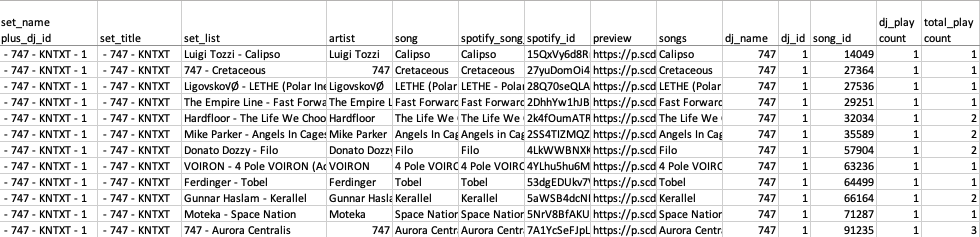
\includegraphics[scale=0.55]{images/dataset}
	\centering
	\caption{Table showing a DJ Set in the dataset} 
\end{figure}

Figure 5.1 shows a DJ Set entry in the dataset. Each song has a link to a preview due to the spotify id being accessible.


\subsection{Initial Suggestions}
The inital suggestions part of the  model is made using Alternating Least Squares, a matrix factorisation algorithm that was made popular by the Netflix Prize award. As explained in chapter 2, this is both an affectively computational way of handling a dataset, and splitting up a matrix to its latent factors reveals trends in between songs and DJs.

A model is made from the dataset, then a list of songs gets inputted. A for loop is ran that will find similar items with the ALS algoritm for each song. the number of recommended song suggestions for each song was set to 200, to assure a large amount of similar songs are used in the next part of the model.

\begin{figure}[H]
	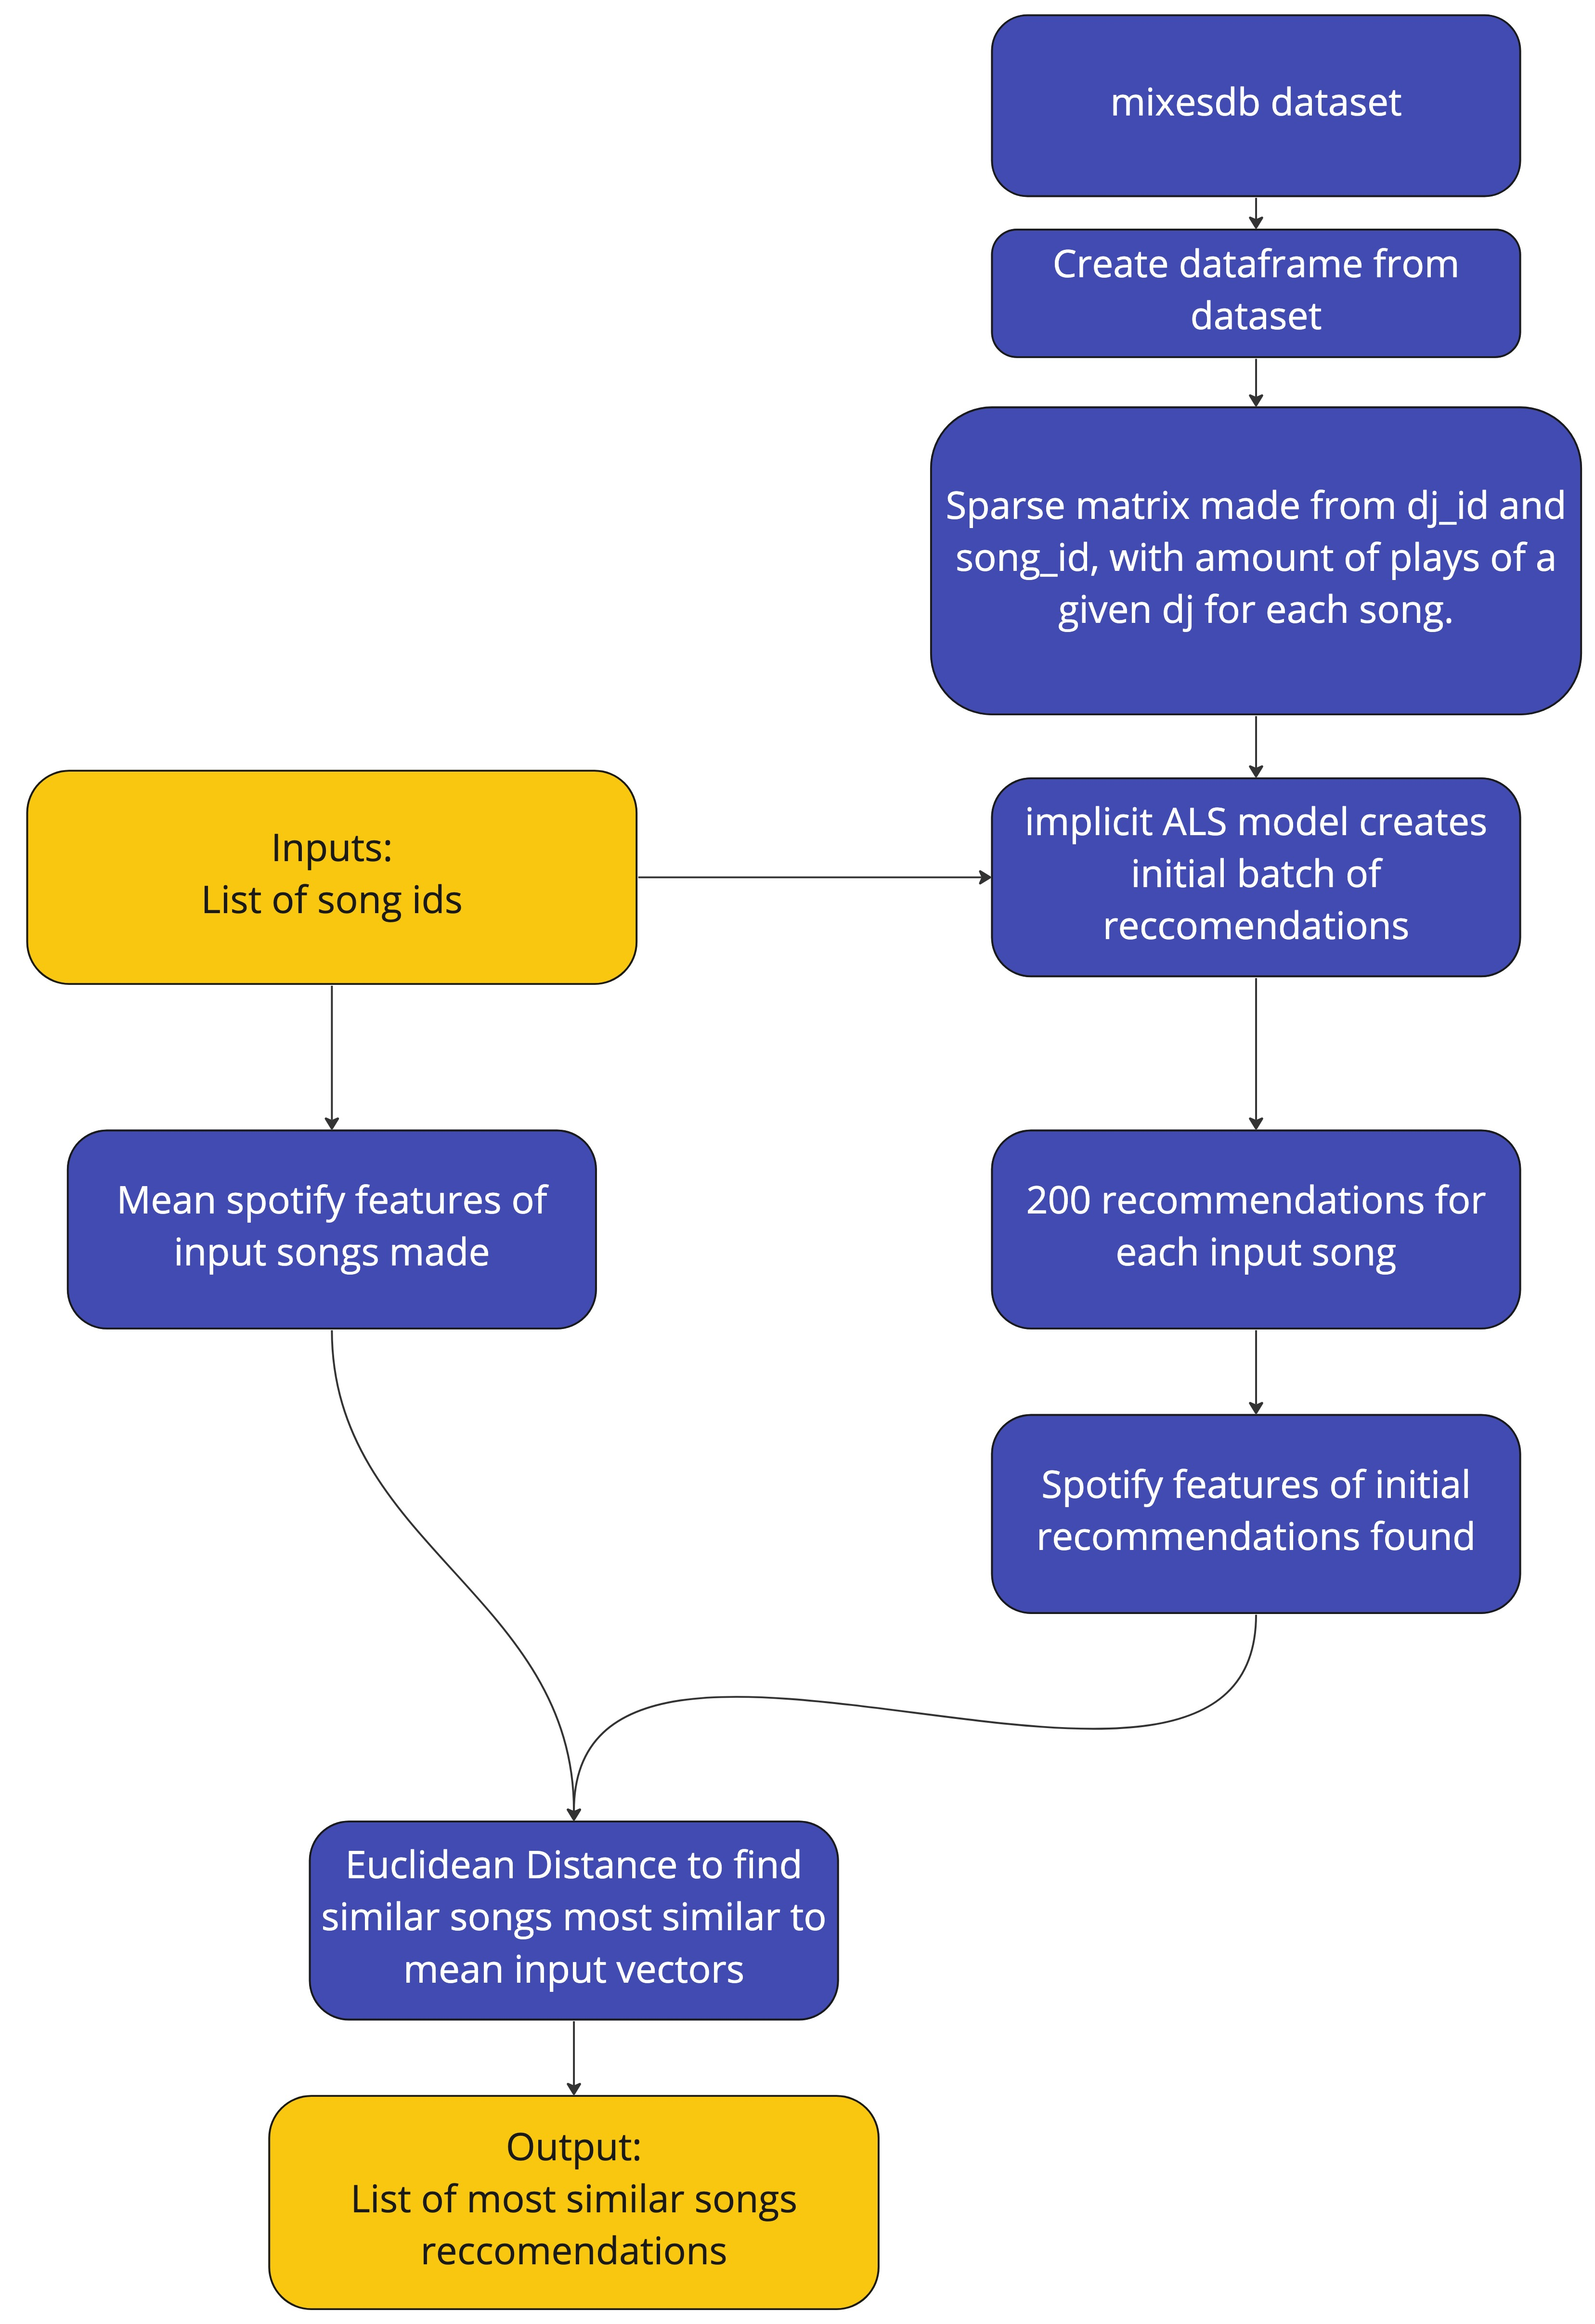
\includegraphics[scale=0.1]{images/application_app_flow}
	\centering
	\caption{Application flow of the application} 
\end{figure}

\subsection{Final Suggestions}
As of yet the code used is similar to Daniel Chows, aside from iterating through many song inputs, instead of one. To add an extra layer of filtering, the spotify API is used to further explore which songs are the most similar.

Using both the input songs, and initital suggestions, using the spotify ID a variety of audio features can be found. They are as listed:

\begin{enumerate}
	\item \textbf{acousticness} - A measure on how acoustic the song sounds (1 being definitely acoustic  )
	\item \textbf{danceability} - Measurement on how suitable a track is for dancing based on tempo, rhythmic features and overall regularity. 1.0 is most danceable. 
	\item \textbf{energy} - a measurement of intensity and activity. Typically, energetic tracks feel fast, loud, and noisy. A heavy metal track would score high, but a Bach prelude would score low. Attribute including dynamic range, perceived loudness, timbre, onset rate, and general entropy will dictate this value. 1.0 is highly energetic
	\item \textbf{instrumentalness} - Predicts whether a track contains no spoken vocals. Songs scoring 1 likely have no vocals. Values above 0.5 represent instrumental tracks.
	\item \textbf{key} - The key the track is in uses following notation 0 = C, 1 = C$\sharp$/D$\flat$, 2 = D. If key cannot be detected then value is set to -1.
	\item \textbf{liveness} - Measurement on whether recording is live. Higher liveness values represent an increased probability that the track was performed live. A value above 0.8 provides strong likelihood that the track is live.
	\item \textbf{loudness} - Loudness of a given track in dB
	\item \textbf{tempo} - The beats per minute of a given track.
	\item \textbf{time\_signature} - Time signature with the following notation, 3 = 3/4, 4= 4/4, 5 = 5/4
	\item \textbf{speechiness} - Detects if song has spoken word, audio books would score 1 and values ranging from 0.3-0.6 would be combination of music and speech.
	\item \textbf{valence} - A measurement of how positive a song is. With scoring's of 1 being extremely positive.
	
\end{enumerate}


% note that \Blindocument has 5 numbered levels, despite setting secnumdepth above. I (and many style guides) would suggest using no more than 3 numbered levels (incl. the chapter), with the option of a fourth unnumbered level.